% TODO translation
% TODO proof-reading
\subsection{First example}

Let's proceed to simple patching task.

\begin{lstlisting}
public class nag
{
	public static void nag_screen()
	{
		System.out.println("This program is not registered");
	};
	public static void main(String[] args) 
	{
		System.out.println("Greetings from the mega-software");
		nag_screen();
	}
}
\end{lstlisting}

How we would remove printing of ``This program is not registered'' string?

Let's finally load IDA:

\begin{figure}[H]
\centering
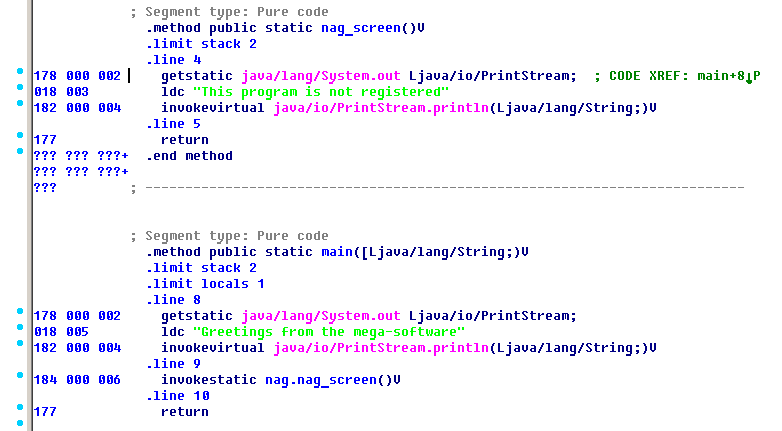
\includegraphics[scale=\FigScale]{Java_and_NET/java/13_patching/1/1.png}
\caption{IDA}
\end{figure}

Let's patch first byte of the function to 177 (which is \TT{return} instruction):

\begin{figure}[H]
\centering
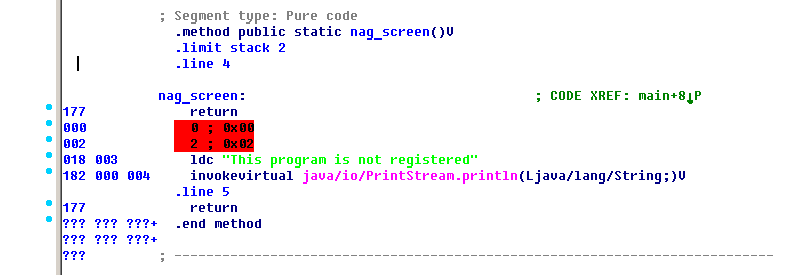
\includegraphics[scale=\FigScale]{Java_and_NET/java/13_patching/1/2.png}
\caption{IDA}
\end{figure}

But that doesn't work (JRE 1.7):

\begin{lstlisting}
Exception in thread "main" java.lang.VerifyError: Expecting a stack map frame
Exception Details:
  Location:
    nag.nag_screen()V @1: nop
  Reason:
    Error exists in the bytecode
  Bytecode:
    0000000: b100 0212 03b6 0004 b1

        at java.lang.Class.getDeclaredMethods0(Native Method)
        at java.lang.Class.privateGetDeclaredMethods(Class.java:2615)
        at java.lang.Class.getMethod0(Class.java:2856)
        at java.lang.Class.getMethod(Class.java:1668)
        at sun.launcher.LauncherHelper.getMainMethod(LauncherHelper.java:494)
        at sun.launcher.LauncherHelper.checkAndLoadMain(LauncherHelper.java:486)
\end{lstlisting}

Perhaps, JVM has some other checks related to stack maps.

OK, let's patch it differently by removing call to \TT{nag()}:

\begin{figure}[H]
\centering
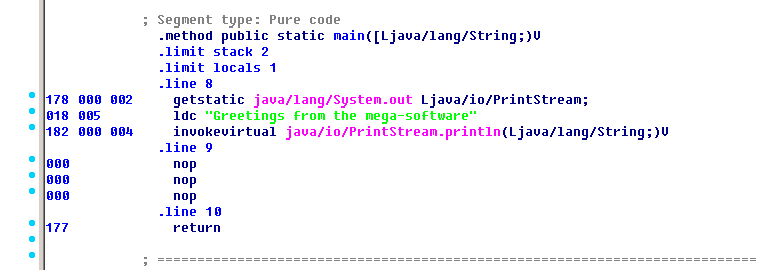
\includegraphics[scale=\FigScale]{Java_and_NET/java/13_patching/1/3.png}
\caption{IDA}
\end{figure}

0 is opcode for \ac{NOP}.

Now that works!
